\setcounter{topnumber}{5}
\setcounter{bottomnumber}{5}
\setcounter{totalnumber}{5}

\chapter{Procedimentos e resultados}

\centerline{\begin{minipage}[c]{\textwidth}
		\centering
		\noindent
		\captionof{figure}{Transistor bipolar atuando como fonte de corrente}
		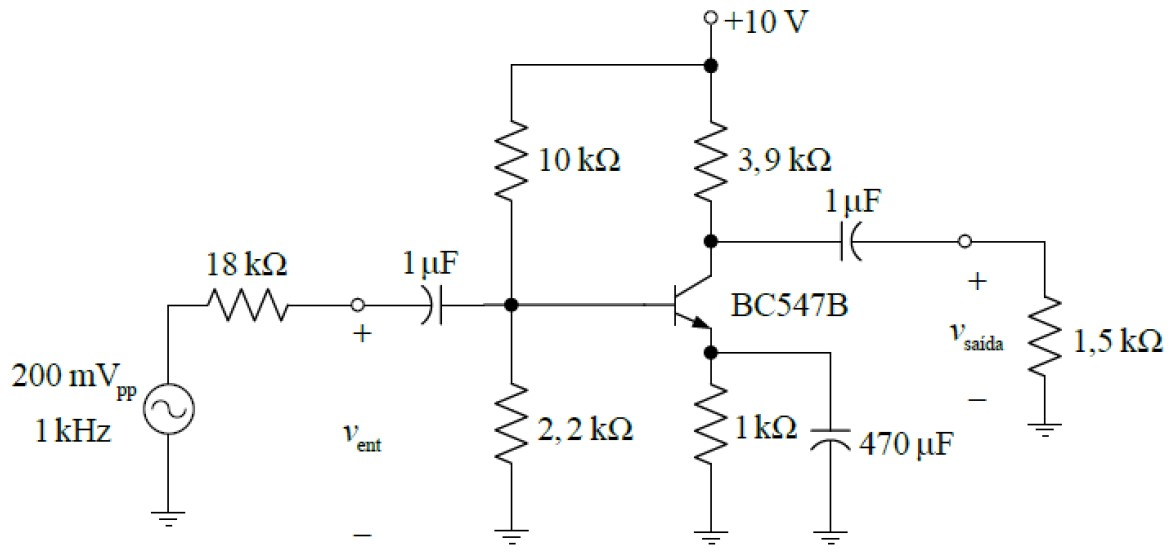
\includegraphics[width=0.5\textwidth]{Imagens/Figura1.jpg}
		\legend{Fonte: Produzido pelos autores}
		\label{Figura1}
\end{minipage}}


\begin{enumerate}
	\item Monte o circuito da Figura \ref{Figura1}, meça as variáveis mostradas na Tabela \ref{Tabela1} e calcule os erros percentuais:

$$\%\; de\; erro = \frac{valor \; prático - valor \; teórico}{valor \; teórico} \times 100$$

	Considerando uma queda de tensão no led em condução de $ 1,5 V $ e de acordo com o datasheet do transistor $ 2N2222 $, temos $ \beta = 150 $, completando assim a Tabela \ref{Tabela1}:

\centerline{\begin{minipage}[c]{\textwidth}
		\centering
		\noindent
		\captionof{table}{Valores teóricos e práticos do circuito da Figura 1}
		\begin{tabular}{cccccc}
			\toprule
			Variável & Valor teórico & Valor prático & Erro (\%) \\
			\midrule \midrule
			$I_{LED}$ &  $ 20mA $ & $ 19,7 mA $ & $1,5 \% $ \\
			\midrule
			$I_{B}$ &  $ 133,33\mu A$ & $ 1,066 mA $ & $ 699 \% $ \\
			\midrule
			$I_{C}$ &  $ 20mA $ & $ 19,69 mA $ & $ 1,55\% $ \\
			\midrule
			$V_{CE}$ &  $ 4,1V $ & $ 2,449 V $ & $ 40,26 \% $ \\
			\midrule
			$\beta$ & $ 150 $ & $ 18,47 $ & $ 87,68 \% $ \\
			\midrule
			\bottomrule
		\end{tabular}%
		\legend{Fonte: Produzido pelos autores}
		\label{Tabela1}
\end{minipage}}

	Com a Tabela \ref{Tabela1}, percebemos uma grande diferença entre o valor teórico e o valor prático, que de acordo com que analisamos, essa grande diferença vem da questão da queda de tensão do LED no teórico foi de $ 1,5V $, sendo que na prática, o LED que usamos tinha a queda de tensão de $ 3,12 V $. E outro motivo para diferenciarem tanto os valores, foi a questão da obtenção do $ \beta $, tendo um valor bem diferente do prático, para efeitos de comparação, refizemos os cálculos teóricos, tendo a queda de tensão do LED com $ 3,12 V $ e o $ \beta $ sendo $ 18,47 $, de acordo com que achamos na prática:
	
	\begin{center}
		\textit{Análise de Malha Coletor-Emissor}
	\end{center}
	
	\begin{center}
		$ -10V+3,12V+V_{CE} +220\Omega\times I_C=0 \Rightarrow V_{CE}=+10V-3,12V-220\Omega(20mA)$
	\end{center}
	
	\begin{center}
		$ \therefore V_{CE}=2,48V $
	\end{center}
	
	Com $ \beta = 18,47 $, temos que:
	
	\begin{center}
		$I_B=\dfrac{I_C}{(\beta+1)}=\dfrac{20mA}{(18,47+1)}=1,027mA $
	\end{center}

	Completando novamente a tabela com os novos dados, lembrando que $ I_C=I_{LED} $, temos:

\centerline{\begin{minipage}[c]{\textwidth}
		\centering
		\noindent
		\captionof{table}{Valores teóricos e práticos do circuito com as alterações}
		\begin{tabular}{cccccc}
			\toprule
			Variável & Valor teórico & Valor prático & Erro (\%) \\
			\midrule \midrule
			$I_{LED}$ &  $ 20mA $ & $ 19,7 mA $ & $1,5 \% $ \\
			\midrule
			$I_{B}$ &  $ 1,027mA$ & $ 1,066 mA $ & $ 3,8 \% $ \\
			\midrule
			$I_{C}$ &  $ 20mA $ & $ 19,69 mA $ & $ 1,55 \% $ \\
			\midrule
			$V_{CE}$ &  $ 2,48 V $ & $ 2,449 V $ &  $ 1,25 \% $ \\
			\midrule
			$\beta$ & $ 18,47 $ & $ 18,47 $ & $ 0\% $ \\
			\midrule
			\bottomrule
		\end{tabular}%
		\legend{Fonte: Produzido pelos autores}
		\label{Tabela2}
\end{minipage}}

	De acordo com Tabela \ref{Tabela2}, temos uma diferença muito menor da prática para o teórico, apresentando os dois valores aproximados.
	
\end{enumerate}